
\begin{itemize}
    \item 
\item  $N free model parameters << N_constraints$
\item  In our specific design this expands to:
\item  $(model parameters + current_value parameter) << N (independent and uncorrelated)$ constraints.
\item  For the different classes of Reduced Model we show that the optimizer converges when data is simulated.


Here I show graphs of
\end{itemize}



In a simulated experiment, existing models were instantiated using a randomly chosen model parameters.

In the class of reduced neural models we are optimizing, are not arbitrary waveform generators. The models have intrinsic restrictions that prevent them from matching perfectly with experimental waveforms.

When constraints are derived from model measurements, intrinsic model restrictions no longer apply. Optimized models should match perfectly with the simulated experiments. 

* Failure to match is indicative of:

- Failure to setup tractable optimization problems.
- When inverting linear equations, finding a unique solution requires that the number of constraining equations is greater than the number of free variables you are solving for:

\section{Pitfalls}
Errors are correlated, and constraints are too few.
To protect against a situation where the collection of error sources guiding optimization are too correlated with each other, to act as 


\section{Verification}
It was important to be able to create a ground truths that were always possible for the optimizer to match exactly. Often experimental data implies waveform shapes that are beyond the capabilities of the model that is to be fitted. Simulating experimental measurements meant, that model limitations can be understood separately from optimizer limitations.

\section{Optimizer Limitations}


\begin{center}
    \begin{figure}
    
        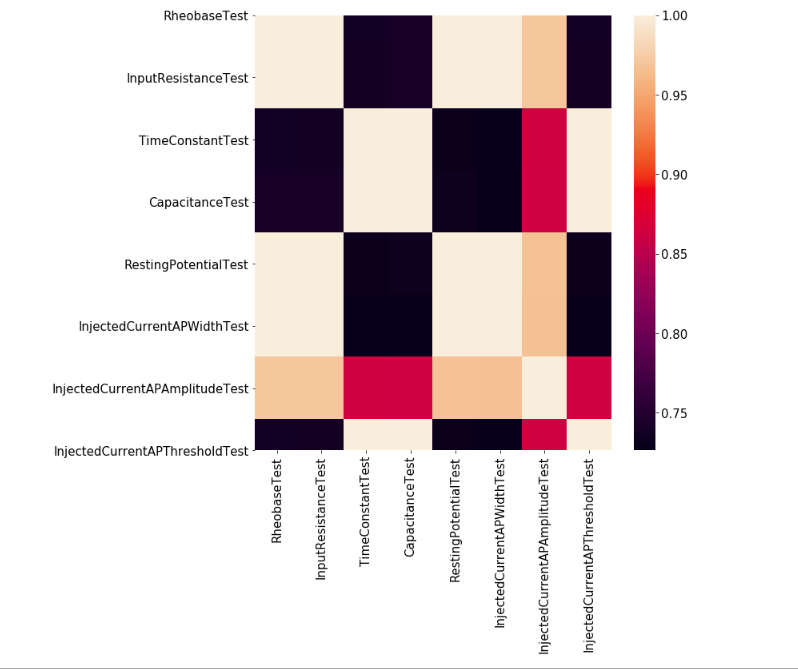
\includegraphics[width=\linewidth]{figures/correlated_errors.png}
    
    	\caption{Test caption}
    \end{figure}
\end{center}